\chapter{تجهیزات پیشنهادی و برآورد هزینه}
\label{chap:cost}
%=====================================================================

\section{مأخذ برآورد}

برآوردهای این فصل بر مبنای قیمت‌های عمومی منتشرشده توسط تولیدکنندگان و گزارش‌های تحلیل بازار جهانی است و \textbf{صرفاً برای برنامه‌ریزی اولیهٔ بودجه} ارائه می‌شود؛ قیمت نهایی باید از طریق استعلام رسمی و مناقصهٔ بین‌المللی/داخلی مطابق مقررات ساماندهی خرید کالای دولتی مشخص شود. لازم به ذکر است که به‌دلیل تحریم‌های فناوری، ممکن است دسترسی مستقیم به برخی تولیدکنندگان غربی (\lr{ID Quantique}، \lr{Toshiba}) با محدودیت مواجه باشد و لازم است گزینه‌های جایگزین (تأمین از طریق کشورهای ثالث، یا توسعهٔ داخلی نمونهٔ اولیه با همکاری مراکز پژوهشی داخلی) نیز به‌موازات ارزیابی شود.

\section{هزینهٔ تجهیزات هر گره}

بر اساس داده‌های صنعتی، هزینهٔ یک زوج سامانهٔ \lr{QKD} تجاری (فرستنده و گیرنده) بسته به نسل فناوری و نرخ کلید، در بازهٔ وسیعی قرار می‌گیرد: نمونه‌های اولیهٔ تجاری در حدود $82000$ دلار برای یک زوج \Cite{mittech2009}، سامانه‌های میان‌رده در بازهٔ $150000$ تا $400000$ دلار \Cite{arxiv0905report}، و آشکارسازهای فوق‌پیشرفتهٔ نانوسیم ابررسانا برای برد بلند در حدود $100000$ یورو برای هر واحد \Cite{techtimes2026sweden}. برای یک شبکهٔ متروپلیتن سازمانی متوسط با دو تا سه سایت در شعاع $50$ کیلومتری، هزینهٔ کل معمولاً بین $500000$ تا $3$ میلیون دلار برآورد می‌شود \Cite{marketintelo2026}.

\begin{table}[htbp]
\centering
\caption{برآورد هزینهٔ اجزای اصلی طرح پایلوت تهران (شش گره، توپولوژی حلقه‌ای)}
\label{tab:cost}
\small
\begin{tabular}{p{5.5cm}p{3.5cm}p{4.5cm}}
\toprule
\textbf{قلم هزینه} & \textbf{برآورد (میلیون دلار)} & \textbf{توضیح} \\
\midrule
سامانه‌های \lr{QKD} (شش زوج فرستنده/گیرنده) & $1.8$ -- $3.2$ & بر مبنای سامانهٔ میان‌رده تا پیشرفته \Cite{idq2025cerberis,toshiba2026qkd} \\
\lr{KMS} و نرم‌افزار مدیریت کلید & $0.3$ -- $0.5$ & شامل مجوز نرم‌افزار و یکپارچه‌سازی \lr{API} \\
فیبر تاریک (اجاره/حفاری تکمیلی) & $0.5$ -- $0.9$ & بسته به میزان فیبر موجود مخابرات ایران \\
رمزگذارهای خط و تجهیزات شبکه & $0.4$ -- $0.8$ & رمزگذار \lr{AES-256} سازگار با \lr{QKD} \\
یکپارچه‌سازی \lr{PQC} در نرم‌افزار بانکی & $0.3$ -- $0.6$ & پیاده‌سازی \lr{ML-KEM/ML-DSA} در زیرساخت پیام‌رسانی بانکی \\
آموزش، ممیزی امنیتی و گواهی‌دهی & $0.2$ -- $0.4$ & شامل آزمون نفوذ و ارزیابی مستقل \\
بهره‌برداری و نگهداشت سالانه (سال اول) & $0.3$ -- $0.5$ & پشتیبانی فنی، پایش و به‌روزرسانی \\
\midrule
\textbf{جمع کل برآوردی (فاز پایلوت)} & \textbf{$3.8$ -- $6.9$} & \\
\bottomrule
\end{tabular}
\end{table}

شکل \ref{fig:costchart} توزیع تقریبی این هزینه‌ها را برای سناریوی میانی نشان می‌دهد.

\begin{figure}[htbp]
\centering
\begin{tikzpicture}
\begin{axis}[
  ybar,
  bar width=16pt,
  width=12.5cm,height=6.5cm,
  symbolic x coords={تجهیزات \lr{QKD},\lr{KMS},فیبر,رمزگذار,\lr{PQC},آموزش,بهره‌برداری},
  xtick=data,
  x tick label style={font=\scriptsize,rotate=20,anchor=east},
  ylabel={میلیون دلار},
  nodes near coords,
  nodes near coords style={font=\scriptsize},
  ymin=0,
  ymajorgrids=true,
  grid style=dashed,
]
\addplot[fill=blue!35] coordinates {
  (تجهیزات \lr{QKD},2.5) (\lr{KMS},0.4) (فیبر,0.7) (رمزگذار,0.6) (\lr{PQC},0.45) (آموزش,0.3) (بهره‌برداری,0.4)
};
\end{axis}
\end{tikzpicture}
\caption{توزیع تقریبی برآورد هزینهٔ فاز پایلوت (سناریوی میانی)}
\label{fig:costchart}
\end{figure}

برای مشاهدهٔ سریع‌تر سهم نسبی هر قلم هزینه از کل بودجه، شکل \ref{fig:costpie} همان داده‌ها را به‌صورت نمودار دایره‌ای نمایش می‌دهد؛ همان‌طور که مشخص است، تنها تجهیزات \lr{QKD} به‌تنهایی نزدیک به نیمی از کل بودجهٔ فاز پایلوت را تشکیل می‌دهد.

\begin{figure}[htbp]
\centering
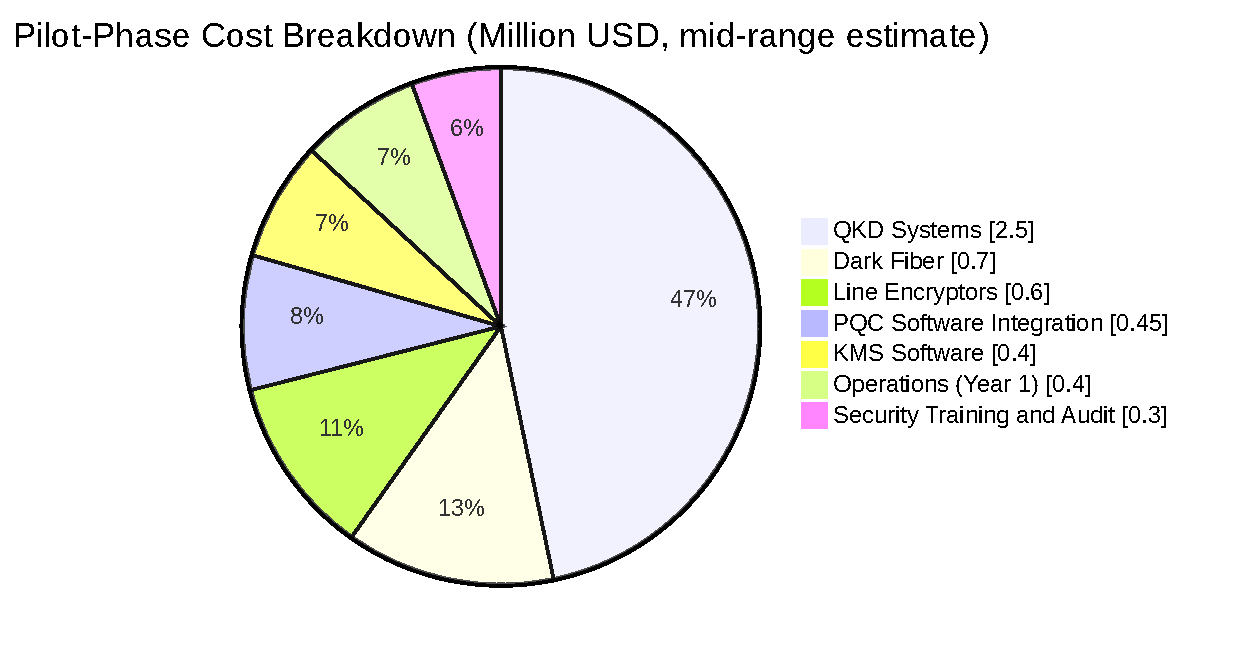
\includegraphics[width=0.72\linewidth]{figs/fig_cost_pie.pdf}
\caption{سهم نسبی هر قلم از برآورد هزینهٔ فاز پایلوت}
\label{fig:costpie}
\end{figure}

\section{هزینهٔ توسعهٔ آتی به مقیاس ملی}

بازار جهانی \lr{QKD} در افق سال $2035$ به حدود $20$ میلیارد دلار برآورد می‌شود \Cite{toshiba2020launch}. توسعهٔ طرح از مقیاس پایلوت کلان‌شهری به یک کریدور بین‌شهری (مثلاً تهران--اصفهان یا تهران--مشهد) نیازمند سرمایه‌گذاری در مقیاس ده‌ها میلیون دلار و افق زمانی چندساله خواهد بود و پیشنهاد می‌شود صرفاً پس از تکمیل موفق و ارزیابی امنیتی فاز پایلوت بررسی شود.

%=====================================================================
